\documentclass[border=8mm]{standalone}
\usepackage{tikz}
\usetikzlibrary{shadows}
\usepackage{pgf-umlcd}
\usepackage{xcolor}
\usepackage[T1]{fontenc}

\definecolor{page}{HTML}{8bd4e0}
\pagecolor{page}

\definecolor{text}{HTML}{3b3b3b}
\definecolor{draw}{HTML}{000000} % {999999}
\definecolor{fill}{HTML}{ededed}

\renewcommand{\umltextcolor}{text}
\renewcommand{\umldrawcolor}{draw}
\renewcommand{\umlfillcolor}{fill}

\begin{document}
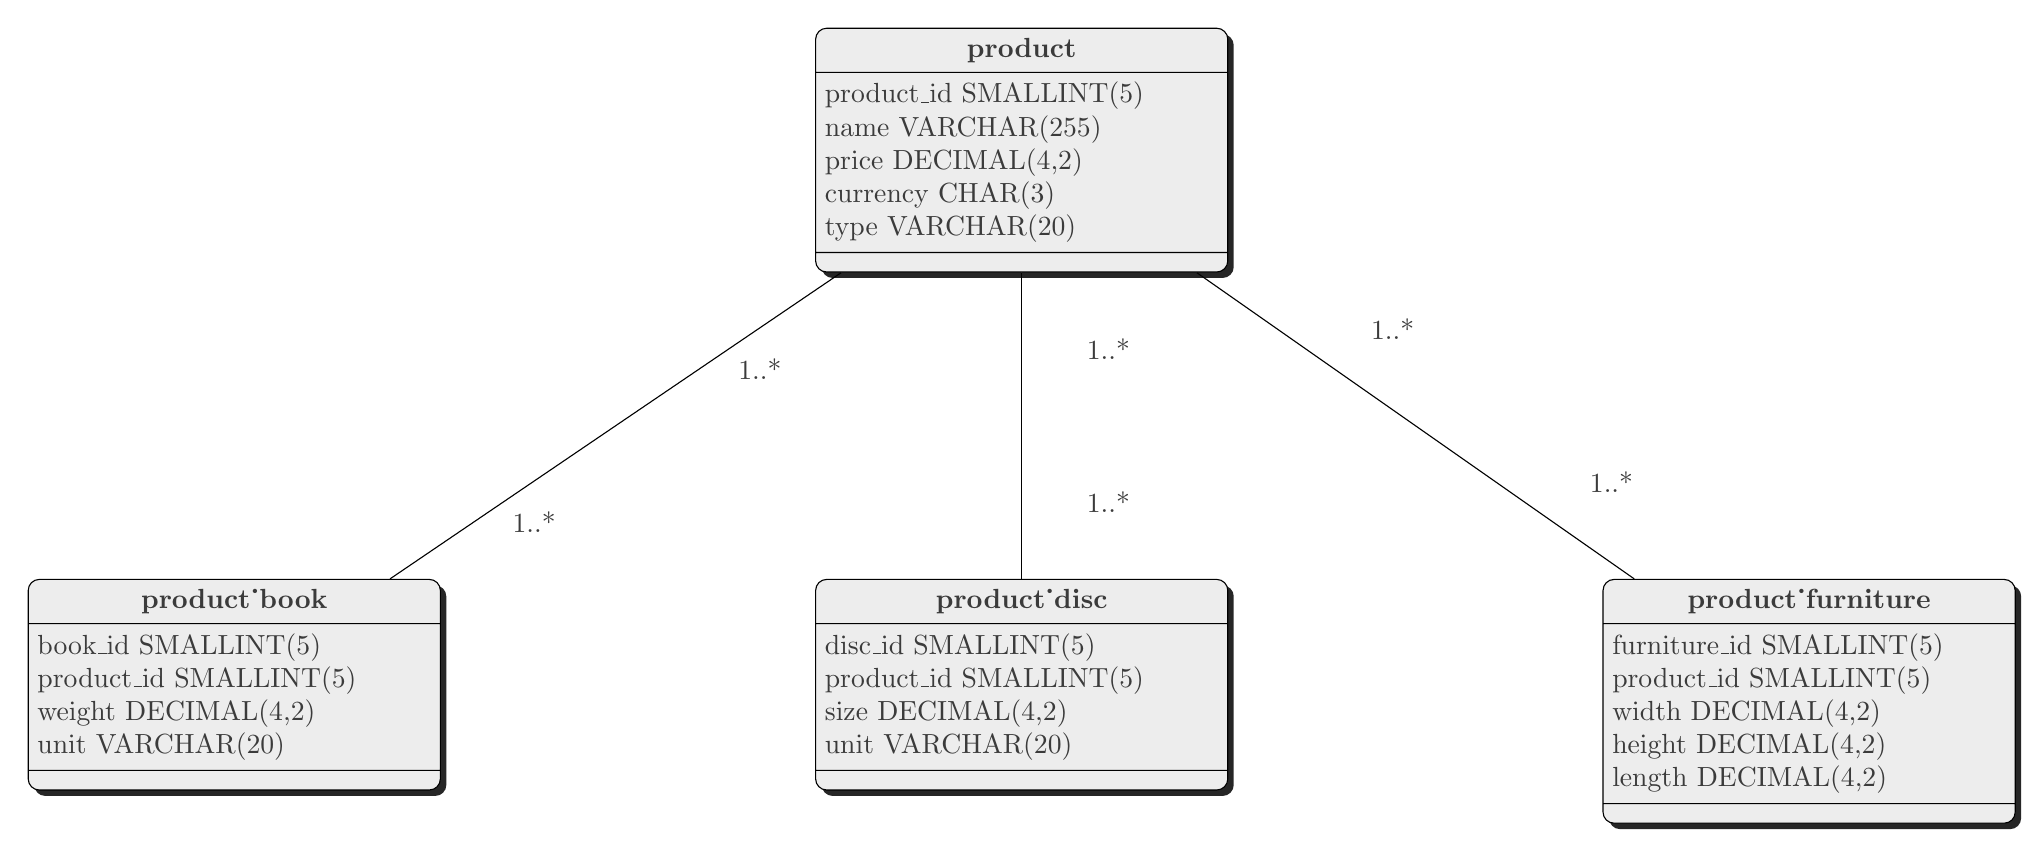
\begin{tikzpicture}[{umlcd style class}/.append style={rounded corners=4pt, drop shadow={opacity=.85, fill=black},}]
\begin{class}{product}{10,0}
    \attribute{product\_id SMALLINT(5)}
    \attribute{name VARCHAR(255)}
    \attribute{price DECIMAL(4,2)}
    \attribute{currency CHAR(3)}
    \attribute{type VARCHAR(20)}
\end{class}
\begin{class}{product\string_book}{0,-7}
    \attribute{book\_id SMALLINT(5)}
    \attribute{product\_id SMALLINT(5)}
    \attribute{weight DECIMAL(4,2)}
    \attribute{unit VARCHAR(20)}
\end{class}
\begin{class}{product\string_disc}{10,-7}
    \attribute{disc\_id SMALLINT(5)}
    \attribute{product\_id SMALLINT(5)}
    \attribute{size DECIMAL(4,2)}
    \attribute{unit VARCHAR(20)}
\end{class}
\begin{class}{product\string_furniture}{20,-7}
    \attribute{furniture\_id SMALLINT(5)}
    \attribute{product\_id SMALLINT(5)}
    \attribute{width DECIMAL(4,2)}
    \attribute{height DECIMAL(4,2)}
    \attribute{length DECIMAL(4,2)}
\end{class}
\association{product}{1..*}{}{product\string_book}{1..*}{}
\association{product}{\quad\quad1..*}{}{product\string_disc}{\quad\quad1..*}{}
\association{product}{\quad\quad1..*}{}{product\string_furniture}{\quad\quad1..*}{}
\end{tikzpicture}
\end{document}
